\documentclass[main.tex]{subfiles}

\begin{document}

\section{Progressive Photon Mapping} \label{section:ppm}

The main problem with the original proposal for photon mapping is that the quality of the final result is limited by the size of the photon map, which in turn has its size limited by the amount of memory available.

Since effects such as caustics are simulated by directly using the information from the photon map, it is necessary to use a very large number of photons in order to avoid noise in the rendering. Thus, the overall accuracy is limited by the available memory. In other words, the accuracy of photon mapping is not only computationally bounded, but also memory bounded, while usual unbiased methods are only computationally bounded.

\cite{hachisuka2008progressive} proposes a progressive approach to photon mapping, which makes it possible to simulate global illumination, including the effects provided by traditional photon mapping, with arbitrary accuracy, and without being limited by memory. This is done by using a multi step algorithm instead of a two step one, where the first pass consists of a ray tracing step to capture a collection of hit points in the scene, and later multiple photon tracing steps are processed iteratively, with each new iteration improving the accuracy of the result in order to converge to an accurate solution, but without storing photon maps from previous iterations.

\image[width=\textwidth]{visio/diagram_ppm}{High Level Fluxogram of Progressive Photon Mapping}{fig:diagram_ppm}

\subsection{First Step: Ray Tracing}

The first step is a standard ray tracing step, used to find all surfaces visible in the scene. Rays are traced through each pixel of the image plane, in order to find all visible surfaces in the scene. For each ray, all hits with a non-specular component in the \acs{BRDF} function are stored. This includes storing the hit location ($x$), the ray direction($\vec{\omega}$) and the pixel it originated from. Additionally, data for the progressive estimation is also included, such as a radius, intercepted flux, and number of photons within the defined radius.


\subsection{Next Steps: Photon Tracing}

After the initial ray tracing step, an iterative process begins. Each iteration, a given number of photons is traced into the scene, building a photon map. At the end, all hit points stored from the initial step are processed, to find all the photons in the map that are within the radius of that hit point. These photons are used to refine the estimate of the illumination of the hit point.

Once this contribution is computed, the photon map is no longer needed, and can be discarded, before the next iteration repeats the process.

This provides two key advantages over the original, two-step approach. The total amount of photons traced is not limited by memory, but only by the amount of iterations that are computed. An arbitrary number of iterations can be used, without requiring any additional memory at all, and resulting in a better quality result. Also, after each photon pass an image can be rendered, and the progressive result can be shown while the image is progressively improved, instead of having to wait for the entire algorithm to finish.

\begin{figure}
  \centering
  \begin{subfigure}{.5\textwidth}
    \centering
    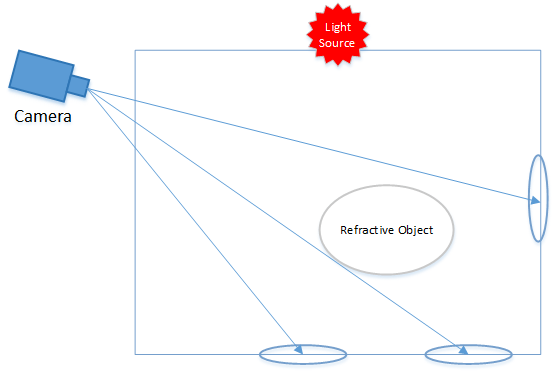
\includegraphics[width=.95\linewidth]{visio/ppm_step1}
    \caption{First step: Ray tracing \label{fig:ppm_step1}}
  \end{subfigure}%
  \begin{subfigure}{.5\textwidth}
    \centering
    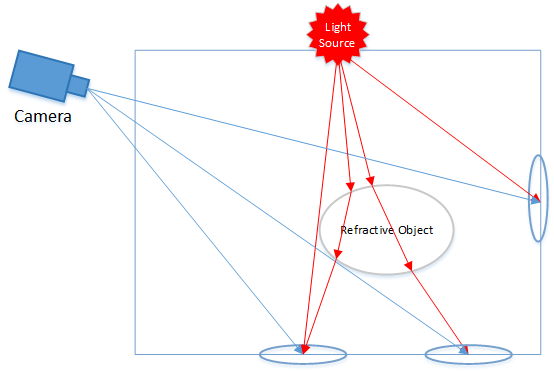
\includegraphics[width=.95\linewidth]{visio/ppm_step2}
    \caption{Next steps: Photon Tracing \label{fig:ppm_step2}}
  \end{subfigure}
  \caption{Overview of Progressive Photon Mapping \label{fig:ppm_overview}}
\end{figure}


\subsection{Radiance Estimation}

Traditional photon mapping estimates radiance by using the density of photons, given by \cref{eq:density}. This is based on locating the nearest $N$ photons within a sphere of radius $R(x)$. The surface are is assumed to be flat, and the surface area is approximated to $\pi R(x)^{2}$. In progressive photon mapping, using this estimation may result in different iterations having different estimations for the same hit point.

\begin{figure}[!htp]
  \begin{equation}
    d(x) = \frac{N}{\pi R(x)^{2}}
  \label{eq:density}
  \end{equation}
\end{figure}

To solve this, the estimations from each iteration can be averaged to obtain a more accurate estimate. However, the final result will not be more detailed than the result of each individual photon map, which is not desirable. Also, as the radius $R(x)$ is constant throughout the iterations, small details within that radius cannot be correctly solved, making the overall accuracy limited by the size of each individual photon map.

The solution to this, also proposed in \cite{hachisuka2008progressive} consists of combining the estimate from each photon map in such a way that the final estimation will converge to a correct solution. The key technique is to reduce the radius $r$ at each hit point, for every new photon map computed.

\subsubsection{Radius Reduction}

Assuming each hit point has a radius $R(x)$, and that $N(x)$ photons have already been accumulated in it, after a new photon tracing step, resulting in $M(x)$ new photons within the radius $R(x)$, the new photon density $\hat{d}(x)$ can be given by \cref{eq:density_new}

\begin{figure}[!htp]
  \begin{equation}
    \hat{d}(x) = \frac{N(x) + M(x)}{\pi R(x)^{2}}
  \label{eq:density_new}
  \end{equation}
\end{figure}

The radius reduction step is about computing a new, smaller radius $\hat{R}(x)$ for each hit point, such that the amount of photons within the new radius $\hat{N}(x)$ is greater that the amount of photons that was present in the previous radius. This ensures that the final result is increasingly more accurate, and converges to a correct solution. The radius reduction is illustrated in \cref{fig:radius_reduction}.

The proposed approach in \cite{hachisuka2008progressive} simplifies this by using a parameter $\alpha$ to control the fraction of photons to keep after an iteration. Therefore, $\hat{N}(x)$ can be given by \cref{eq:photon_count_new}.

\begin{figure}[!htp]
  \begin{equation}
    \hat{N}(x) = N(x) + \alpha M(x)
  \label{eq:photon_count_new}
  \end{equation}
\end{figure}


\image[width=0.7\textwidth]{radius_reduction}{Radius Reduction after a Photon Tracing step}{fig:radius_reduction}

The final radius $\hat{R}(x)$ can be computed by combining \cref{eq:density,eq:density_new,eq:photon_count_new}, and as shown by the original work on the subject, can be given, for each single hit point, by \cref{eq:radius_new}.

\begin{figure}[!htp]
  \begin{equation}
    \hat{R}(x) = R(x) - dR(x) = R(x) \sqrt{\frac{N(x) + \alpha M(x)}{N(x) + M(x)}}
  \label{eq:radius_new}
  \end{equation}
\end{figure}

\end{document}
